
\chapter{Introduction}

Time series is an important category of data, since climate, finance, and health data all can be structured as time series. Classical regression, clustering and classification of time series data often works by analysing the observed values directly. Ordinal Patterns(OPs) take a different approach to time series analysis.
Instead of using the observed values, OPs transform those values into symbols.
These symbols retain information about the relative values, and aspire to capturing relevant information about the time series and the process that produced it.

Ordinal Patterns have been around for twenty years.
They were proposed by Bandt and Pompe in 2002~\cite{Bandt2002}.
This seminal article has received, to date, over \num{3000} citations on the Web of Science.
Their main properties are invariance, robustness, and being model-agnostic.

OPs have been used in applications in several domains.
Many of these applications involve comparing time series, signals, and images through features extracted from their Ordinal Patterns.
Since results about the distribution of such features are recent, our initial interest was comparing existing conclusions with those supported by the new statistical tests.
While approaching this research avenue, we found indications of reproducibility crisis~\cite{Fidler2018} in this field, mostly related to data availability.
We then moved into the application of these new tests to already published results, and found evidence of the other type of reproducibility crisis: diverging results depending on the type of library employed.
MAGNUS; then, we decided to study the effect of preprocessing of the data by a combination of omitting Na values and adding noise to break ties. A new tie breaking method is proposed and its performance on computing entropy and p values is investigated.

We are interested in verifying the reproducibility of results of Ordinal Patterns in the scientific literature.
Initially, we wanted to check how many of the 3000 articles, were reproducible. This was a big task, so at first it was narrowed down to just papers focusing on climate. In the end, around 31 papers were investigated deeply.

\chapter{Ordinal Patterns}

\section{History}
Bandt and Pompe's first paper about ordinal patterns is from 2002. 
They introduced the concept of turning a time series or signal into a sequence of symbols. 
They furthermore used the Shannon entropy on the symbol distribution~\cite{Bandt2002}. 
The Shannon Entropy was developed in 1948 by C.\ E.\ Shannon~\cite{Shannon1948} as a way to quantify uncertainty and unpredictability.

The 1995 paper ``A statistical measure of complexity'' by López-Ruiz et al.~\cite{LopezRuiz1995} introduced the concept of a statistical measure of complexity. 
This idea was applied to OPs in 2003~\cite{Martin2003}, and in 2004 the version of it using Jensen-Shannon divergence was published~\cite{Lamberti2004}.
We use the latter in this work.

\section{Definition}

Every analysis that employs OPs starts by defining the (integer-valued) word size $D\in\{2,3,\dots\}$ and time lag $\tau$.
We will only use $\tau=1$, and thus will drop, it from the following discussion.

Consider the finite time series of real values $\bm x=(x_1, x_2,\dots, x_{n+D-1})$. 
The word size $D$ is chosen, as seen in the bibliometric analysis below, a word size between 3-6 is most common.
The Bandt \& Pompe transformation (also called ``BP Symbolisation'') converts each subset of size $D$ of contiguous and different values into a symbol, i.e.,
the first tuple of $D$ values will be $(x_1,x_2,\dots,x_{D})$, 
the second tuple will be $(x_2, x_3,\dots,x_{D+1})$, and so on.

There are at least two ways of computing OPs.
We will describe one of them.
Each tuple is transformed into a pattern by ranking them by numerical order. 
The lowest observation gets assigned the number $0$ and the highest observation gets the number $D-1$. 
The pattern can then be written as a string of these numbers. 
The tuple $(0.51, 0.79, 0.14)$ will have pattern $1,2,0$.
How we write the patterns is transparent, provided there is only one pattern for each possible sorting of the tuple.
For example, we could have defined that $(0.51, 0.79, 0.14)$ becomes $\pi^3$ or $c$ or $\mathfrak{c}$.
Assuming there are no ties in each word, there are $D!$ possible patterns that we will denote $\bm\Pi=\{\pi^1,\pi^2,\dots,\pi^{D!}\}$.

By applying the BP symbolisation, we transform the time series 
$\bm x = (x_1, x_2, \dots, x_{n+D-1})$ into the sequence of symbols
$\bm \pi = (\pi_1, \pi_2,\dots, \pi_n)$.
The observed frequency pattern $\widehat{p}_i$ is defined as
$$
\widehat{p}_i=\frac{\#\{t : \pi_t = \pi^i\}}{n} ,
$$
with which we define the vector of observed proportions:
$$
\widehat{\bm p} = (\widehat{p}_1, \widehat{p}_2, \dots, \widehat{p}_{D!}).
$$



A tie is when a tuple contains identical values. In practice, there may be ties, for instance when observing times series registered with finite precision.
There are several ways to handle ties.
They can be ignored, i.e., no pattern is computed for tuples with ties,
or they can be broken by adding small random perturbations. 
Techniques that handle ties are usually referred to as ``imputation solutions.''

OPs are usually considered useful for time series of at least length $n>100D$.

\begin{figure}
    \centering
    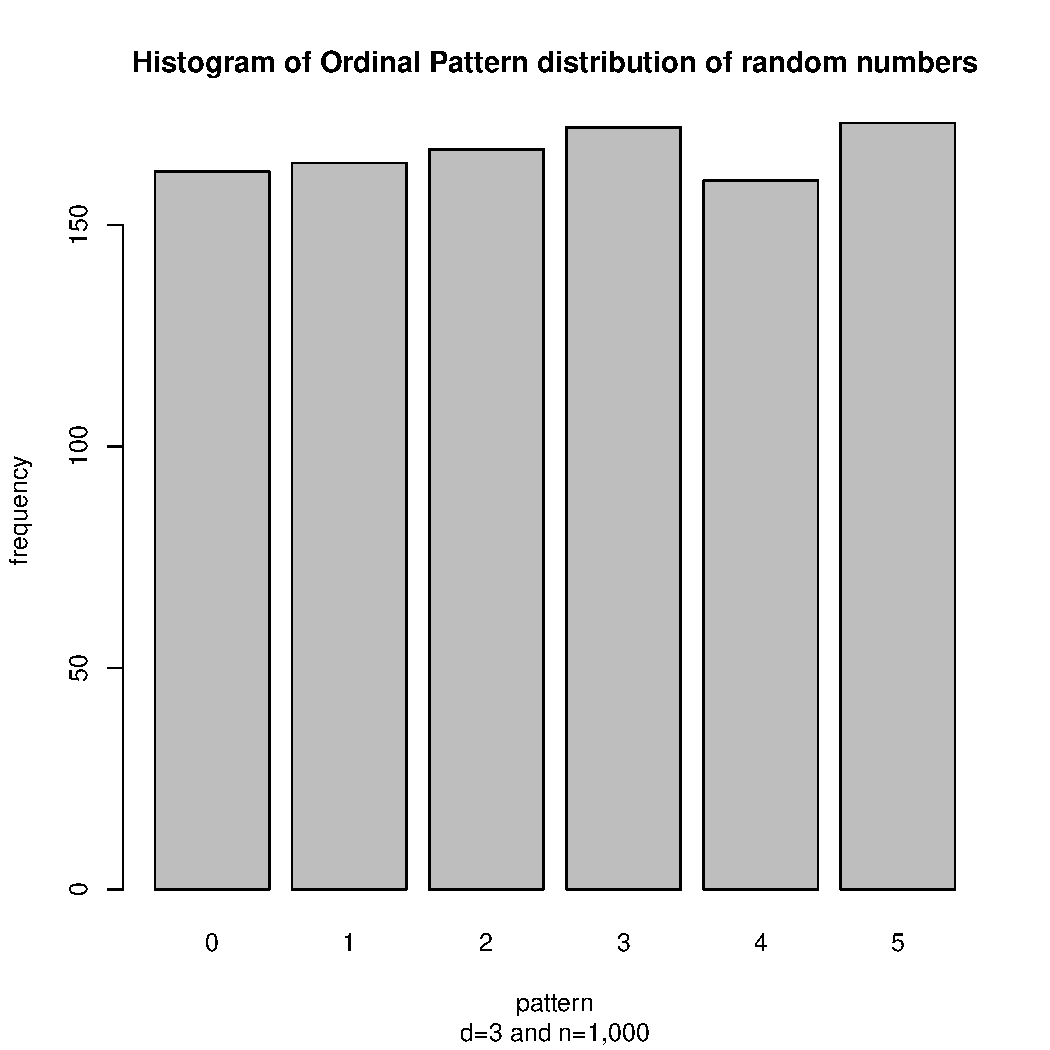
\includegraphics[width=\textwidth,keepaspectratio]{./powerlaw/histogram.pdf}
    \caption{Simple histogram of the ordinal pattern distribution of random numbers}
\end{figure}

From the ordinal pattern distribution, features can be extracted. The two main used features in this field are Entropy and Complexity. In this paper, Shannon Entropy will be used, which is defined as.

$$h(n)=-\sum p(\pi) \ln(p(\pi))$$
Normalized version
$$H(n)=-\frac{\sum p(\pi) \ln(p(\pi))}{\ln(D!)}$$

There are several statistical complexity measures that can be used. They are all a product between the used entropy and a distance measure. In this paper Martin-Plastino-Rosso intensive Statistical Complexity Measure is used, where the distance measure is Jensen-Shannon divergence, and it is measured between the pattern distribution and the uniform distribution. The $Q_0$ is normalizing term. It is defined as

$$C[\mathscr{P}]=H[\mathscr{P}]\cdot Q_J[\mathscr{P},\mathscr{P}_e]$$

$$Q_J[\mathscr{P},\mathscr{P}_e]=Q_0\cdot \mathscr{J}[\mathscr{P},\mathscr{P}_e]$$

$$\mathscr{J}[\mathscr{P},\mathscr{P}_e]=S[\frac{\mathscr{P}+\mathscr{P}_ee}{2}]-S[\frac{\mathscr{P}}{2}]-S[\frac{\mathscr{P}_e}{2}]$$

$$\mathscr{P}_e=\{p_j=\frac{1}{W};j=1...,W\}$$
$$Q_0 = -2(\frac{W+1}{W}ln(W+1)-2ln(2W)+ln(W))^{-1}$$
\cite{Amigo2023b}

\paragraph{Applications}
Going to the original Bandt and Pompe paper \cite{Bandt2002} on Semantic Scholar and getting the ten most recent citations, gives a good picture of how broadly this methodology is being used.

The topic varies from: "Walnut crack detection..." \cite{Zhang2024}, Schizophrenia \cite{Wang2024}, Analysis of Smart Drilling \cite{Szwajka2024}, Epileptic Seizure detection \cite{AbhishekParikh2024}, mind wandering during video-based learning \cite{Tang2024} and Random Numbers generated based on dual-channel chaotic light \cite{Liu2024}. The rest that was found \cite{Demirel2024, Du2024, Sun2024, Li2024}

\section{Reproducibility}
\paragraph{Reproducibility crisis}
In data science, data from many scientific fields are analysed, as shown in the application section of ordinal patterns above. It therefore increases the difficulty of reproducing the data collection stage, as most cases requires an interdisciplinary study involving multiple people. In some cases it is impossible e.g. if the equipment needed is unavailable or a time series of weather data cannot be recollected, since it is impossible to go back in time. The point of science is to eliminate trust, when sharing knowledge, however the above observations highlights the need for some degree of trust, in cases, where data cannot be reproduced. Only data that is random numbers, generated in a script, will be reproduced in this paper.

The COVID pandemic gave birth to the following quote. "We warn against the potential misuse or misleading interpretation of public data of variable quality" \cite{Struelens2021}. Data from different governments does not have the same quality. This necessities good source criticism. In this paper data from peer-reviewed studies will be trusted, which have often either produced the data themselves or got it from reputable organizations as NASA or NOAA. 

In this paper, the focus will be on direct computational reproduction.

"Computational reproducibility is most often direct (reproducing particular analysis outcomes from the same data set using the same code and software), but it can also be conceptual (analysing the same raw data set with alternative approaches, different models or statistical frameworks)" \cite{Fidler2018}

\section{Bibliometric analysis}
31 articles were analysed for data availability and used word size. The majority of them are about climate, and they explicit have to used Permutation Entropy. Four categories were made for data availability: “Available”, “Sourced”, “On-Request” and “not Available”. Sourced is the broadest category. Some articles give a detailed description of how to pull the data from a website. Other articles give no description, expect, which organisation they got the data from. The is no differentiation between these cases in the category S. A is the best category and only used, when the data is directly downloadable. R is when the dataset has to be requested by the author and is suboptimal. N is the worst category, because there is no source to data, nor is the dataset attached to the paper in any way. Word size between 2-7 were used. Some articles used multiple word sizes, which is why the sum of “No. articles using” is higher than 31. Only 4 articles were the data readily downloadable. The data is definitely possible to get from some articles in category "S", but many of them were very sparse in their description of the data, to the point, where it would be hard to pull it from the website. Assuming that around half of the data from articles in "S" can be pulled from their sources. That leaves around 50\% of the article, where it is not possible to reproduce the data processing part of the article. Ideally, all papers should be reproducible and especially their data processing part, since modern technology allows for extremely efficient data sharing across vast distance to a very affordable price. According to this paper~\cite{Baker2016} more than 70\% of researches have failed reproducing an article and 52\% agree that there is significant reproducibility crisis. In this paper, cases occurred, where the data had been downloaded and verified to being true, but the data processing could not be reproduced.


\begin{table}[]
\begin{tabular}{|l|l|l|l|l|l|l|l|}
\hline
Word size & 2 & 3  & 4  & 5 & 6 & 7 & Mutliple \\ \hline
No. articles using  & 4 & 13 & 15 & 9 & 6 & 1 & 9        \\ \hline
\end{tabular}
\end{table}

\begin{table}[]
\begin{tabular}{|l|l|l|l|}
\hline
A & S  & R & N \\ \hline
4 & 19 & 3 & 4 \\ \hline
\end{tabular}
\end{table}

\begin{figure}
    \centering
    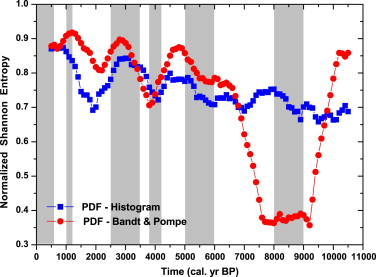
\includegraphics[width=\textwidth,keepaspectratio]{ElNino/ArticleEntropyPlot.jpg}
    \caption{Original papers entropy plot, Red dots should be equal to the dots in plots below}
\end{figure}

\begin{figure}
    \centering
    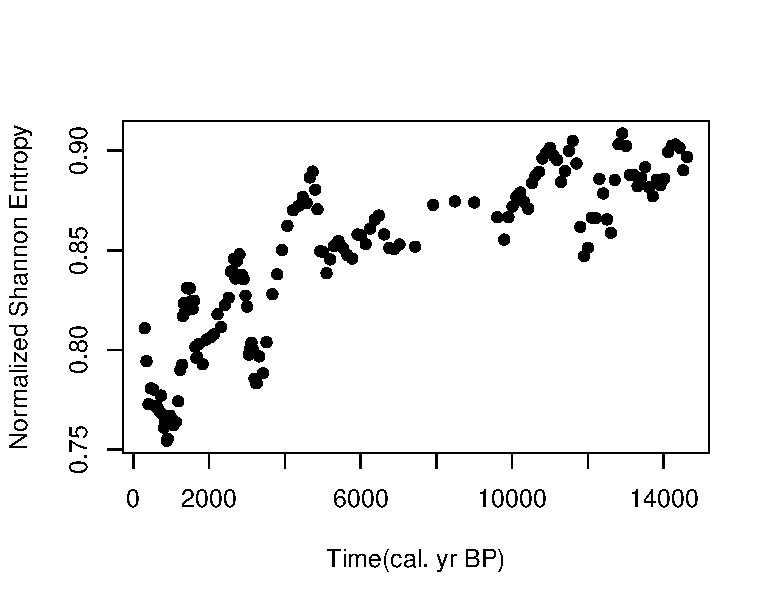
\includegraphics[width=\textwidth,keepaspectratio]{ElNino/Entropy.pdf}
    \caption{This papers reproduction. The x-axis is slightly bigger, however the data in range 0-11,000 cal. yr BP, where verified to be identical, and that is not identical in any way.}
\end{figure}